%% 	This LaTeX Template is meant for "Second Bachelor´s Thesis"
%% 	written by Frank A Titze in March 2009
%% 	for Hochschule Kufstein Tirol, Austria, Dep. Wirtschaftsinformatik
%% 	www.hsk-edu.at
%% 	@author Frank A Titze (frank.a.titze@gmx.eu)
%% 	@copyright 2009, FAT
%% 	@license GPL
%% 	@version 1.0
%%=================================================
%% 	Main Document  Vorlage_BA2_by.fat.tex
%% 	This document:  mainmatter.tex
%%=================================================

%% Hier soll der Hauptteil der Arbeit erscheinen
%% auskommentieren der folgenden Zeile entfern den Beispielcontent
%% %% 	This LaTeX Template is meant for "Second Bachelor´s Thesis"
%% 	written by Frank A Titze in March 2009
%% 	for Hochschule Kufstein Tirol, Austria, Dep. Wirtschaftsinformatik
%% 	www.hsk-edu.at
%% 	@author Frank A Titze (frank.a.titze@gmx.eu)
%% 	@copyright 2009, FAT
%% 	@license GPL
%% 	@version 1.0
%%=================================================
%% 	Main Document  Vorlage_BA2_by.fat.tex
%% 	This document:  beispiele.tex
%%=================================================

%% Zusätzliche Trennvorschriften:
\hyphenation{op-tical net-works semi-conduc-tor e-com-merce Top-Ma-na-ge-ment}


\chapter{Beispielcontent}


\section{Quellenverweise}

Die Sache mit dem Zitieren ist eine Geschichte voller Missverständnisse. Zuerst gibt es da nämlich die Unterscheidung zwischen Kurz- und Langzitaten.

Ein sogenanntes Kurzzitat ist ein Verweis im Text, der auf Autorenname(n) und Jahreszahl besteht \cite[vgl.][S.72]{Jarz2008}. Es ist uns freigestellt, ob wir wie hier den Literaturverweis direkt in den Text einbauen wie in einschlägiger Literatur meist anzutreffen, oder -- wie es dem Herrn Jarz ganz gut gefällt -- über Fußnoten unsere Quellenangaben machen. Für die Sache mit den Fußnoten habe ich deshalb auch etwas eingebaut\footcite[S.39]{Jarz2008}. 

Ein Lang- oder Vollzitat hingegen ist eine komplette Quellenangabe, so wie wir es ins Quellenverzeichnis hinten im Dokument schreiben. So etwas stünde immer in einer Fußnote, ist meines Erachtens aber überflüssig, da wir ja ein Quellenverzeichnis haben. Daher sollten Verweise im Text ausreichen.\footcite{paula}

Um die Formatierung des Quellenverzeichnis übrigens müssen wir uns nicht weiter kümmern, solange alle relevanten Daten über JabRef in der Literaturdatenbank eingetragen sind, \BibTeX~ sei Dank.







\section*{Sectionüberschrift ohne Nummerierung}
Hier eine Sectionüberschrift ohne Nummerierung: Das geht auch mit anderen Überschriften, und liegt an dem angefügten Stern im Code.



\section{Liste mit Punkten}
\begin{itemize}
\item Punkt1 mit Text
\item Noch etwas
\item Und was ganz anderes
\item Ebenso ein Schmarrn
\end{itemize}



\section{Nummerierte Liste}
\begin{enumerate}
\item Punkt1 mit Text
\item Noch etwas
\item Und was ganz anderes
\item Ebenso ein Schmarrn
\end{enumerate}



\section{Liste Description}
\begin{description}
\item[davor] Punkt1 mit Text
\item[lalala] Noch etwas
\item[huhuu] Und was ganz anderes
\item[undso] Ebenso ein Schmarrn
\end{description}



\section{Ein Bildchen}
Ein Verweis auf ein Bild (wie z.B. Abbildung~\ref{fig:texlogo} auf Seite~\pageref{fig:texlogo} ) im geschriebenen Text wird immer per Nummerierung gemacht, nie mit einem Doppelpunkt nach einem Satz der vor dem Bild zu stehen hat. 

\begin{figure}[!t]
	\centering
			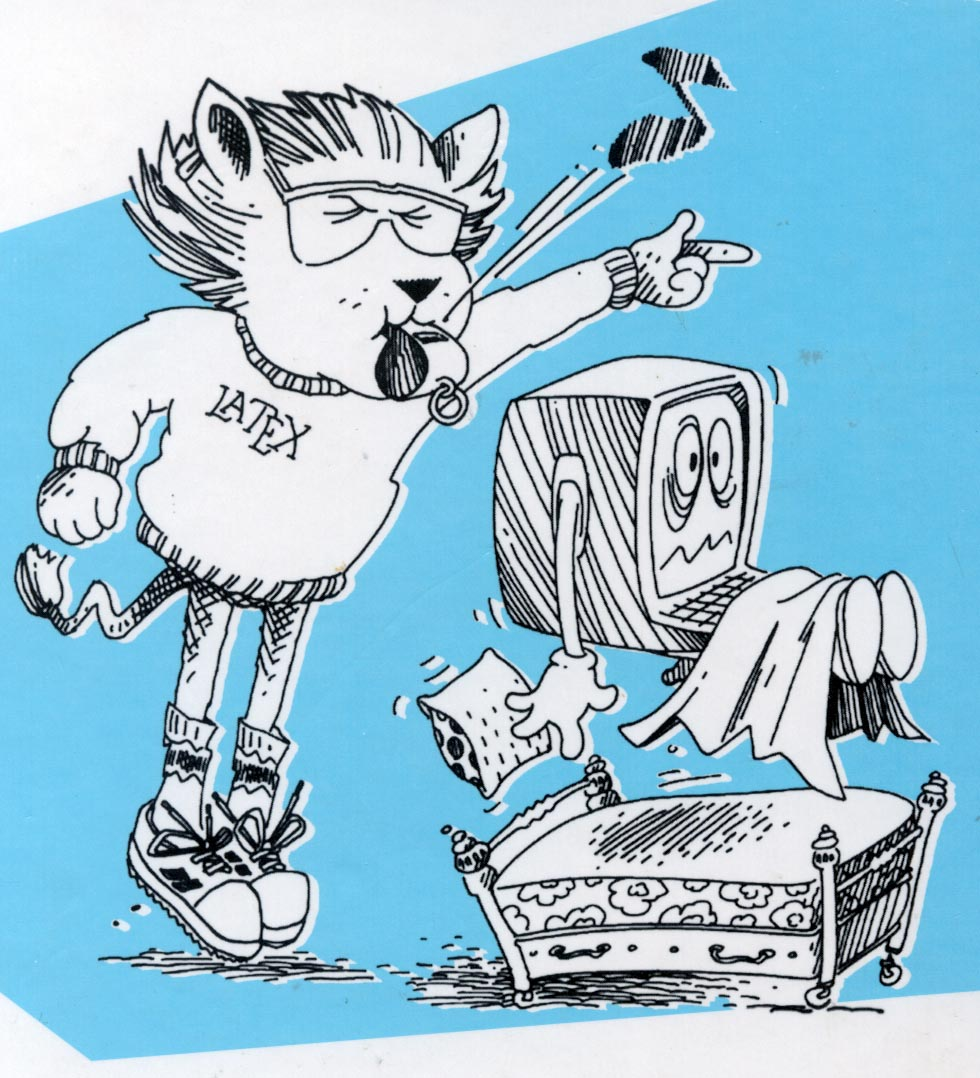
\includegraphics[width=0.5\textwidth]{misc/latex.jpg} 		% Bild relativ zur Textbreite skalieren
	   	  \caption[\LaTeX~Logo] % Dieser Text hier erscheint im Abbildungsverzeichnis
	   	  				{Und dieser Text hier erscheint schlussendlich direkt unterhalb des Bildes. Daher kann hier durchaus auch etwas mehr stehen.}
  			\label{fig:texlogo}
\end{figure}






\section{Textformatierungen}

In diesem Text werden ein paar wenige, aber übliche Formatierungen dargestellt,
je nachdem ob man \textbf{fett} drucken möchte, \textit{kursiv} oder \underline{unterstrichen}, aber auch die \emph{Hervorhebung}
gewisser Terme könnte von Vorteil sein.

Obacht! Fettdruck im normalen Fließtext sollte NIEMALS nötig sein\footcite[S.112]{Jarz2008}.

Gerade für Sourcecode bietet sich die \texttt{Schreibweise mit fester Laufweite} an. Für Namen würde sich eventuell auch
die Verwendung echter \textsc{Kapitälchen} anbieten, für welche ganz explizit \LaTeX~sehr bekannt ist.

Termini technici werden oft auch \textsl{slanted} oder \textit{kursiv} dargestellt, mit kleinen Unterschieden.

\section{Ein herausgestelltes Zitat}
\begin{zitat}
		"`Graecum te, Albuci, quam Romanum atque Sabinum,
		municipem Ponti, Tritani, centurionum,
		praeclarorum hominum ac primorum signiferumque,
		maluisti dici. Graece ergo praetor Athenis,
		id quod maluisti, te, cum ad me accedis, saluto:
		'chaere,' inquam, 'Tite!' lictores, turma omnis chorusque:
		'chaere, Tite!' hinc hostis mi Albucius, hinc inimicus."'
\end{zitat}





\section{Eine einfache Tabelle}

Tabellen werden in der table-Umgebung gesetzt, um auch als Tabellen erkannt zu werden (siehe Tabelle~\ref{tab:WerkCicero} auf Seite~\pageref{tab:WerkCicero}). Fügte man hier beispielsweise das Bild oder PDF einer Excel-Tabelle ein, würde es ebenso  als Tabelle geführt. 

\begin{table}[!t]
	\centering
	\begin{tabular}{cll}\hline\hline
	Jahr & Originaltitel & engl. Titel \\ \hline
	84 BC & De Inventione & About the composition of arguments \\
	55 BC & De Oratore & About oratory \\
	54 BC & De Partitionibus Oratoriae & About the subdivisions of oratory \\
	52 BC & De Optimo Genere Oratorum & About the Best Kind of Orators \\
	46 BC & Paradoxa Stoicorum & Stoic Paradoxes \\
	46 BC & Brutus & For Brutus \\
	46 BC & Orator ad M. Brutum & About the Orator, dedicated to Brutus \\
	45 BC & De Fato & On Fate \\
	44 BC & Topica & Topics of argumentation \\ \hline\hline
	\end{tabular}
	\caption[Dies ist der Kurztitel fürs Verzeichnis]{Und hier steht dann derjenige Text, welcher direkt unterhalb der Tabelle zu finden ist.}
	\label{tab:WerkCicero} 	% Textmarke
\end{table}






\section{Verweise und Referenzen}
\label{sec:references}
Indem man \verb+\label+ im Code vergibt, kann man mit \verb+\ref+ direkt darauf verweisen, und mit \verb+\pageref+ sogar die Seitennummer angeben. Als Rückgabewert kommt bei Bildern und Tabellen die jeweilige Nummerierung, bei Überschriften die Gliederungsnummer. An dieser Stelle verweise ich auf Überschrift~ \ref{sec:references}, welche auf Seite~ \pageref{sec:references} steht.

Die Tilde im Code bedeutet, dass an dieser Stelle ein fester Leerraum steht, der nicht getrennt werden darf.




\section{Sourcecode einfügen}
Sourcecode wird in der \verb+\listings+ Umgebung gesetzt, mit vielen Möglichkeiten der Formatierung. Es wird fast jede Programmiersprache explizit unterstützt. Näheres unter \url{http://www.pvv.ntnu.no/~berland/latex/docs/listings.pdf}


\begin{lstlisting}[caption=Dies ist ein PHP Beispiel]{Beispiel}
public function delete(){
  if($_SESSION["loginstat"] == "v33PL")
  {
   $this->db_delete("bbericht", "IDbbericht", $_GET["id"], "");
  }else{
   $this->sec_msg();
  }
}
\end{lstlisting} 	%$ (Dieses Dollarzeichen ist nur eingefügt, da der Editor sonst denkt man hätte hier noch eine mathematische Formel-Umgebung offen, die zwischen Dollarzeichen gesetzt würde)




\section{Silbentrennung}

Sollte \LaTeX~wirklich einmal Probleme mit der Silbentrennung eines unbekannten Wortes haben, kann man über hyphenation
die Trennweise bekannt machen, oder auch das Trennen von Wörtern verbieten.
\begin{verbatim}
\hyphenation{er-go-no-mic} 		
\hyphenation{fortran}
\end{verbatim}
 "`fortran"' darf nie getrennt werden, "`ergonomic"' an den angegebenen Stellen






\section{Mathematische Formeln}
\LaTeX~ ist berühmt für seine einzigartigen Fähigkeiten im Umgang mit mathematischen Formeln.

Dabei gibt es die einfache Variante kurze Formeln wie $1+1=3$ direkt in den Text einzufügen, oder auch komplexere Formeln herausgehoben darzustellen, die dann auch nummeriert werden:

\begin{equation}%Beginn der Formel
t-t_{0}=\sqrt{\frac{l}{g}}\int_{0}^{\varphi}{\frac{d\psi}{\sqrt{1-k^{2}\sin^{2} {\psi}}}} = \sqrt{\frac{l}{g}} F(k,\varphi)
\end{equation}%Ende der Formel

\begin{equation}%Beginn der Formel
u(x,t)= 8 \frac{k_{1}^{2}e^{\alpha_{1}} + k_{2}^{2}e^{\alpha_{2}} + (k_{1}-k_{2})^{2}e^{(\alpha_{1}+ \alpha_{2})} \left[2 + \frac{1}{(k_{1} + k_{2})^{2}} ( k_{1}^{2}e^{\alpha_{1}} + k_{2}^{2}e^{\alpha_{2}}) \right]}{\left[1+e^{\alpha_{1}} + e^{\alpha_{2}} + \left(\frac{k_{1} - k_{2}}{k_{1}+k_{2}} \right)^{2} e^{\alpha_{1}+ \alpha_{2}} \right]^{2}}
\end{equation}%Ende der Formel






\section{Anführungszeichen}
Ein Satz mit "`Anführungszeichen"'.
Ein Satz mit französischen \frqq Anführungszeichen\flqq.
Ein Satz mit \textit{halben} französischen \frq Anführungszeichen\flq.



\section{Umlaute}
Sollten mal Probleme mit Umlauten auftreten, kann man sich mit den nativen Umlautzuweisungen behelfen:
\"a, \"A, \"o, \"O, \"u, \"U



\section{Abkürzungen}
Werden im Text Abkürzungen wie \gls{ad} für Active Directory benutzt, müssen diese vorher in der glossary-Datei definiert werden.
Von den zuvor definierten Abkürzungen werden aber nur diejenigen wirklich im Verzeichnis aufgeführt, welche auch im Texr verwendet wurden.
\gls{ad} wurde bereits verwendet mit \verb+\gls{ad}+. Ebenso \gls{ms}, aber CD wurde hier nicht als Code eingefügt, und fehlt daher im Verzeichnis.

Das besondere dabei: Bei der ersten Verwendung im Text wird die Abkürzung automatisch ausgeschrieben! Auch wird das Verzeichnis automatisch alphabetisch sortiert.




\section{Gliederungsebenen}
Die oberste Ebene ist das chapter, hier befinden wir uns gerade in einer section.
\subsection{Subsection}
\subsubsection{Subsubsection}
Spätestens hier sollte man mit Nummerierung aufhören!
\paragraph{Paragraph}
Und wer hier noch Nummerierung will, ist krank ;-)
\subparagraph{Subparagraph}




\section{Blindtext mit \LaTeX}
\lipsum





%%EOF@fat



 	% Einbinden der Beispiele


\chapter{Einleitung}
\label{ch:Einleitung}
Dieses Kapitel gibt eine Einführung in das Thema der Bachelorarbeit. Dabei wird auf die Ausgangssituation und den Aufbau der Arbeit eingegangen. Des weiteren wird die Problemstellung der Arbeit definiert und die Relevanz des Themas beschrieben.


\section{Ausgangssituation}

Anfangs war das Internet lediglich eine Informationsquelle für den Menschen. Mitte der 2000er-Jahre trat eine Veränderung ein. Internetnutzer wollten Teil des Webs werden, selbst Inhalte generieren und mit anderen Internetnutzern teilen. So entwickelte sich das Internet zu einem interaktiven Web, welches unter dem Begriff des \glqq Web 2.0\grqq  durch Tim O'Reilly wesentlich geprägt wurde\footcite{oreilly}.

Auch hat die Zahl der Mobiltelefone in den letzten 15 Jahren sehr stark zugenommen.
Heutzutage sind Mobiltelefone und Internetzugang aus unserem alltäglichen Leben nicht mehr wegzudenken. Aus dem Mobile Communications Report 2017 der Mobile Marketing Assosiation Austria und der MindTake Research geht hervor, dass Stand 2017 bereits 94\% der Österreicher ein Smartphone besitzen. 93\% der Österreicher nutzen das Internet regelmäßig auf ihrem Smartphone und in der Altersklasse der 15- bis 29-Jährigen, sind es sogar 100\%. Die tägliche Nutzung liegt bei über drei Stunden pro Tag\footcite{MMAA}.

Die schnell voranschreitende Entwicklung neuer Technologien bietet Menschen sehr viele Möglichkeiten zu kommunizieren und sich mit anderen Menschen auszutauschen. Auch sind Menschen nicht mehr an das Internet zu Hause gebunden, sie können mobiles Internet auf ihren Mobiltelefonen, Tablets und Wearables unterwegs nutzen und live Informationen einholen. Die Endgeräte sind leistungsfähiger, benutzerfreundlicher, transportabeler und intelligenter als je zuvor.

Bergsportlern stehen zahlreichen mobile Applikationen, Internetforen, Plattformen und Blogs für die Tourenplanung zur Verfügung. Touren können online angeschaut und geplant werden. Auf Interessensplattformen und Blogs beschreiben Bergsportler ihre eigenen Touren und berichten über ihre  Erlebnisse. Sie schreiben persönliche Reiseberichte mit vielen Details welche von anderen Internetnutzern gelesen und kommentiert werden können. Eine Interaktion zwischen Verfasser und Lesern entsteht. Diese Berichte können Bergsportlern als Motivation und Inspiration für zukünftige Touren dienen. Hier kann jedoch ein Problem lauern, denn nicht jeder Bergsportler ist gleich fit und gleich erfahren.


\section{Problemstellung}

Das Angebot für Tourenplanung ist sehr groß, es reicht von gedruckten Tourenführern über Online-Plattformen zu GPS-fähigen Wearables. Bergtouren können heutzutage besser den je geplant werden. Online-Tools und mobile Applikationen geben Auskunft über die Distanz, Höhenmeter, Beschaffenheit der Strecke und Einkehrmöglichkeiten. Auch das Wetter ist jederzeit zeitnah abrufbar. Dennoch lässt sich der Presseaussendung vom Januar 2018 des österreichischen Kuratoriums für alpine Sicherheit entnehmen, dass die Zahl der unverletzten Bergsportler, welche einen alpinen Notruf absetzten, in den vergangenen 10 Jahren stetig anstieg. Im Jahr 2017 machten Unverletzte bereits 37\% aller Notrufe aus. Alpine Notrufe werden nicht ausschließlich von tatsächlich Verunfallten oder Verletzten abgesetzt, sondern auch von unverletzten Personen, die sich in einer misslichen Lage befinden\footcite{kurasi}.
Um im weiteren Verlauf bessere Aussagen treffen zu können, widmet sich diese Arbeit den Wanderern. Wandern ist der beliebteste Bergsport und wird von Personen jeden Alters und Geschlechts ausgeübt.
In einer Statistik der letzten 10 Jahre kann man entnehmen, dass die Zahl der Unverletzten von 425 im Zeitraum 01.11.2007 bis 31.10.2008 auf 811 im Zeitraum 01.11.2015 bis 31.10.2016 sich fast verdoppelte (siehe Abbildung \ref{fig:uwan}). Die häufigsten Ursachen für einen Notruf von Unverletzten Personen sind {\glqq Verirren und Versteigen\grqq} gefolgt von {\glqq Erschöpfung\grqq}  und {\glqq Wettersturz\grqq}. Es gibt durchaus Faktoren, die nicht vorhersehbar sind. Dazu gehören Wettersturz, Blitzschlag, Steinschlag oder Herz-Kreislaufstörungen. Viele Faktoren können jedoch mit richtiger Vorbereitung und Planung durchaus minimiert werden. Recht hohe Zahlen $($zwischen 41 und 105$)$ findet man unter dem Kriterium {\glqq Sonstiges\grqq}. Das bedeutet, dass keines der angegebenen Kriterien für das Absetzen eines Notrufes des Unverletzten zutraf. Hier stellt sich die Frage, ob es sein kann, dass der technische Fortschritt und die Menge an konsumierten Online-Inhalten dazu führt, dass sich Wanderer nach einer Planungsphase und während der Ausübung der Sportart zu sehr in Sicherheit wiegen und sich eher für zu schwierige Touren entscheiden?
\begin{figure}
	\centering
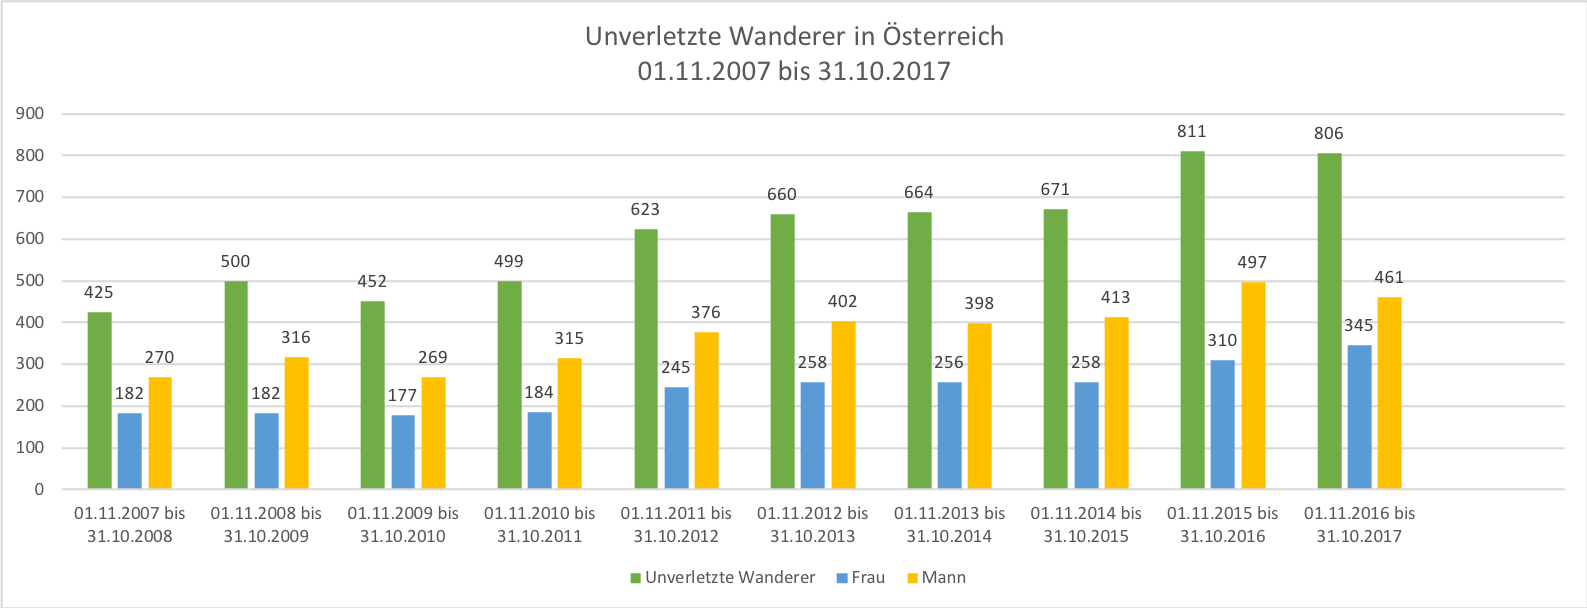
\includegraphics[width=1\linewidth]{content/uwan}
\caption{Unverletzte Wanderer, die in den letzten zehn Jahren einen Notruf absetzten}
\label{fig:uwan}
\end{figure}



\section{Zielsetzung und Forschungsfrage}


Das Ziel der Bachelorarbeit ist es zu erforschen, wie weit  Wanderer von neuen Technologien und konsumierten Online-Inhalten bei der Risikobewertung einer Bergtour beeinflusst werden. Dabei soll einerseits untersucht werden, wie gut Wanderer, die ihnen zur Verfügung stehenden Technologien anwenden. Andererseits wird erforscht, wie Wanderer mit Online-Inhalten umgehen und die nützlichen Informationen filtern und mit ihren Fähigkeiten abgleichen. In einer qualitativen Umfrage soll herausgefunden werden, welche Technologien und Online-Inhalte Wanderer bevorzugt nutzen, um sich ein Bild von einer Tour zu machen. Des Weiteren soll herausgefunden werden, welchen Online-Inhalten Wanderer vertrauen und welche Inhalte für die Entscheidungsfindung welche Tour tatsächlich gegangen wird, herangezogen werden.\\
Daraus lässt sich folgende Forschungsfrage ableiten: 
\textit{Wie werden Wanderer von Online-Inhalten und neuen Technologien bei der Risikobewertung einer Tour beeinflusst?}

\section{Aufbau der Arbeit}

Die vorliegende Bachelorarbeit \textit{Analyse des Entscheidungsverhaltens von Bergsportlern bei der Risikobewertung bei der Auswahl der Route beim Ausüben von Bergsport mit Zuhilfenahme von mobilen Applikationen und Online-Inhalten} besteht aus \# \# \# \# \# \# \# \# Kapiteln.\par

Im ersten Kapitel soll an das Thema der Arbeit herangeführt werden, die Relevanz und Problemstellung werden erläutert und eine Zielsetzung inklusive der Forschungsfrage werden dargestellt.\par

Die Kapitel \# \# \# \# \# \# \# \# enthalten die theoretischen Grundlagen.\par

In \# \# \# \# \# \# \# \# Kapitel wird die Forschungsmethodik erläutert\par

In \# \# \# \# \# \# \# \# Kapitel werden die Ergebnisse vorgestellt und die Arbeit schließt mit einem Fazit und Ausblick in \# \# \# \# \# \# \# \# Kapitel ab.

\chapter{Grundlagen}
\label{ch:Grundlagen}

Im folgenden Kapitel werden die grundlegenden Begriffe, welche für die Bachelorarbeit relevant sind, erläutert. 

\section{Web 2.0}
\label{web2.0}

Das Internet wurde in seinen Anfängen für Informations- und Darstellungszwecke benutzt. Dieses Konzept wird als Web 1.0 bezeichnet. Im Web 1.0 gibt es nur wenige Content-Ersteller. Die überwiegende Mehrheit der Internetnutzer agiert lediglich als Konsument von Inhalten\footcite{unterschiedWeb1u2}. Darauf folgte Anfang der 2000er Jahre das Konzept des Web 2.0. Der Begriff wurde von O'Reilly geprägt, wobei der Begriff bereits zuvor in Gebrauch war. Web 2.0 beschreibt keine neue Technologie sondern vielmehr eine veränderte Nutzung des Internets. O'Reilly beschrieb das Web 2.0 als eine Reihe von Prinzipien und Praktiken, die wie ein Sonnensystem von Websites miteinander verbunden sind, wobei einige oder alle dieser Prinzipien in unterschiedlichem Abstand vom Kern sind\footcite{oreilly}. O'Reilly sieht das Web 2.0 als eine von allen nutzbare Plattform mit Fokus auf datenbasierte Dienste.
Die Trennung, ob eine Internetseite eine Web 1.0 oder Web 2.0-Seite ist, lässt sich nur bei der Analyse mehrerer Achsen sichtbar machen. Dazu muss man sich die technische, strukturelle und soziologische Achse anschauen. Bei der technischen Achse betrachtet man die Präsentationstechnologie, die sowohl zur Darstellung der Webseite als auch zur Interaktion mit dem Benutzer verwendet wird. An der strukturellen Achse wird der Zweck und das Layout der Seite betrachtet und auf der soziologischen Achse werden die Freunde und Gruppen betrachtet\footcite{unterschiedWeb1u2}. \\
Durch die neu entstandene kollaborative Zusammenarbeit ist es möglich, das Wissen vieler Internetnutzer der Allgemeinheit zugänglich zu machen. Somit haben sich Webseiten im Web 2.0 so verändert, dass sie für die interaktive und kollaborative Nutzung die geeigneten Plattformen zur Verfügung stellen und die Webseiten laufend durch die Nutzerbeteiligung auf dem aktuellen Stand gehalten werden. Durch die Nutzerbeteiligung wurden Webseiten und deren Inhalte dynamischer und flexibler.
Durch neue Technologien und das Verlangen des Internetnutzers, seine Erfahrungen, Kenntnisse und Gedanken mitzuteilen, entstand eine neue Interaktivität.


\subsection{Social Web}

Während das Internet genutzt wurde, um die soziale Interaktion zu erleichtern, ermöglichte die Entstehung und schnelle Verbreitung von Web 2.0-Funktionalitäten im ersten Jahrzehnt des 21. Jahrhunderts einen Evolutionssprung in der sozialen Komponente der Webnutzung\footcite[S. 745-750]{obarSocialMedia}. Das Internet hat sich von einem Abrufmedium zu einem partizipativen Mitmachmedium\footcite{panke} entwickelt. Das Social Web kann als Teilbereich des Web 2.0 gesehen werden. WAS ENTWICKELTE SICH? VERSTEH DEN NÄCHSTNE SATZ NICHTEs entwickelte sich, da immer mehr Menschen Zugang zum Internet hatten und die Bedeutung des Internets zunahm sowie dem sozio-technischen Wandel der Netznutzung\footcite[S. 350]{griesbaum}. Einen erheblichen Teil zur Etablierung brachten die geringen technischen Anforderungen hinsichtlich des Betriebes und der Nutzung von Social Software, dazu gehören Programme und Anwendungen. Die Nutzung dieser Software wurde leichter, sodass sie nicht mehr nur von Experten bedient werden konnte. Dies erleichterte die Erstellung von Inhalten und den sozialen Austausch.

Ebersbach et al. teilen das Social Web in die folgenden vier Bereiche ein\footcite[S. 35-36]{ebersbach}:

\begin{itemize}
	\item \textbf{Informationsaustausch:} Beim Informationsaustausch geht es um die Verteilung von Objekten, die gewisse Informationen beinhalten.  Dies können Texte, Videos, Bilder, Fotos, usw. sein.
	\item \textbf{Beziehungsaufbau:} Beim Beziehungsaufbau stehen die zwischenmenschlichen Beziehungen im Fokus. 
	\item \textbf{Kollaborative Zusammenarbeit:} Die kollaborative Zusammenarbeit besteht aus der Sammlung und Herstellung von neuem Wissen, Aussagen und Erkenntnissen. Hier schließen sich Menschen zu Gruppen zusammen und bearbeiten ein von ihnen ausgewähltes Themengebiet.
	\item \textbf{Kommunikation:} Bei der Kommunikation geht es um den Mitteilungsaustausch zwischen Personen.
\end{itemize}


\subsection{User-Generated Content}

Das Web 2.0 hat vielen Nutzern neue Möglichkeiten eröffnet. Einer dieser Möglichkeiten wird User Generated Content (UGC) genannt, also von Nutzern kreierte Inhalte. Genauer wird UGC üblicherweise als: Medieninhalte, die von der Allgemeinheit, statt von bezahlten Professionellen, kreiert oder produziert werden und hauptsächlich im Internet gefunden werden\footcite{terry}, beschrieben. UGC ermöglicht es allen Internetnutzerinnen und -nutzern ihre eigenen Inhalte zu veröffentlichen, sodass andere Nutzer auf diese Inhalte reagieren und antworten können\footcite{cox}. Vor allem in einem Marketingkontext wird UGC auch manchmal als das Word-of-Mouth des Internets oder auch als elektronisches Word-of-Mouth\footcite{morrison} bezeichnet.

UGC kann über unzählige Kanäle und in unzähligen Formen veröffentlicht werden. Dabei kann es genauso auditive (z.B.: Podcasts, Lieder) wie auch visuelle (z.B.: Text, Bilder) oder auch audiovisuelle (z.B.: Video) Gestalt annehmen. Genauer gesagt, spricht man bei UGC am häufigsten über Blogs, Social Media, Produktbewertungen und über kollaborative Enzyklopädien wie Wikipedia\footcite{chen}. UGC ist also ein weites, im Kontext des Internets beinahe allumfassendes, Feld.

Dabei interessiert sich sowohl die Wirtschaft als auch die akademische Forschung vor allem für markenbezogene Inahlte, sogenannten \textit{branded content}. Dies kommt vermutlich daher, dass UGC einen Umbruch im Marketing begonnen hat. Traditionell fand markenbezogene Kommunikation als Einwegnachrichten vom Unternehmen an den Konsumenten statt, die durch die Interessen der Unternehmen typischerweise voreingenommen war\footcite{ramirez}. Heute ermöglicht es jedoch, das interaktive Internetnutzerinnen und -nutzer, ihre Meinung anderen direkt und weniger voreingenommen, mitteilen können. Deshalb wurde UGC eine beliebte Quelle für markenbezogene Information, sodass auch Unternehmen UGC inzwischen große Beachtung schenken\footcite{ramirez}. Insbesondere Interessant ist UGC als qualitatives Feedback für Marken und Unternehmen sowie für authentische, möglichst positive PR oder Werbung. Besonders die Tourismusbranche wird sehr von UGC beeinflusst, wobei Bewertungen, wie zum Beispiel auf Hotelvergleichsseiten oder Reiseblogs sehr wichtig sind\footcite{akehurst}.

\subsection{Vertrauenswürdigkeit von User Generated Content}

Generell kann man von drei Arten von Teilnehmern an UGC sprechen: jene, die hauptsächlich Inhalte selbst kreieren, die sogenannten \textit{Posters}, jene, die Inhalte hauptsächlich passiv konsumieren, die \textit{Lurkers} und jene, die bevorzugt beides tun, die \textit{Networkers}\footcite{morrison}. Hier stellt sich die Frage, was diese drei Typen motiviert, UGC zu veröffentlichen beziehungsweise zu konsumieren. Resultate einer Studie zeigen, dass Altruismus eine große Rolle beim Posten von Inhalten spielt, genau wie ökonomische Anreize oder Vorteile\footcite{poch}. Aber auch das Bedürfnis, dazuzugehören, sein Leben zu teilen und mit anderen Menschen zu interagieren dürfte einflussreich sein\footcite{akehurst}. Das Konsumieren kommt dagegen aus einem Gefühl des Vertrauens. Wie zuvor angedeutet, haben einfache Konsumenten weniger Grund, ein Unternehmen beziehungsweise ein Produkt gut darzustellen, als das Unternehmen selbst. Außerdem kann man davon ausgehen, dass die jeweiligen Posters das Produkt oder den Service schon getestet haben\footcite{akehurst}. Deshalb vertrauen auch rund 68\% aller Konsumenten online Empfehlungen, auch wenn sie die Person nicht direkt kennen\footcite{ramirez}. Darüber hinaus nimmt bei 20\% der Konsumenten UGC einen großen Einfluss auf ihre Urlaubspläne, sodass Konsumenten UGC mehr vertrauen als zum Beispiel professionellen Reiseführern\footcite{akehurst}.

Jedoch gibt es wiederholte Besorgnis, dass UGC keine verlässliche Quelle für konstruktive Informationen ist. Das liegt zu einem Großteil an der Anonymität, die das Internet ermöglicht. Ganz egal, ob es sich um eine Empfehlung, eine Kritik oder sonstiges handelt, man kann nur selten zuverlässig bestimmen, wer hinter einem Inhalt steckt. Gerade dadurch ist es möglich, dass sowohl absichtlich als auch unabsichtlich fehlerhafte Inhalte verbreitet werden können. Angestellte eines Unternehmens können Inhalte manipulieren um besser dazustehen oder die Konkurrenz schlecht zu machen. Manche Nutzer dagegen veröffentlichen Inhalte nach bestem Wissen und Gewissen, haben aber nicht die nötige Kompetenz für ein Thema und verbreiten auf diese Art und Weise ebenfalls Fehlinformationen\footcite{chen}.

Zusammenfassend ergibt sich in User Generated Content eine Möglichkeit für Konsumenten, authentische Meinungen und Empfehlungen sowohl zu veröffentlichen als auch zu konsumieren. Dies macht es für viele Unternehmen interessant, besonders in einem Tourismuskontext, jedoch gibt es auch Gründe, die Zuverlässigkeit von UGC anzuzweifeln.

\section{Mobile Applikationen und mobile Web-Applikationen}

Wie bereits in der Ausgangssituation dieser Arbeit erläutert, sind Mobiltelefone und Internetzugang aus unserem alltäglichen Leben nicht mehr wegzudenken. Aus diesem Grund steigt auch das Angebot und die Nachfrage nach mobilen Applikationen. Diese können per Smartphone oder Tablett heruntergeladen werden um sie überall verwenden zu können. Die angebotenen Applikationen können von kleinen Dienstprogrammen, die nur eine kleines Problem lösen bzw. nur eine Funktion haben, bis hin zu großen Programmpaketen, welche komplexe Funktionen haben, reichen. Die Anzahl der Applikationen in den jeweiligen Appstores ist heutzutage schier unüberschaubar. Die Applikationen müssen nach dem zu Grunde liegendem Betriebssystem, auf dem sie laufen müssen, ausgesucht werden. Die zwei größten Betriebssysteme sind Android und iOS, wobei Android im Mai 2018 einen weltweiten Marktanteil von 76,53\% und iOS von 18,97\% hatte\footcite{mobileos}. In Österreich sind die Zahlen etwas anderes, doch auch hier hat Android laut einer Statistik aus März 2018 einen Marktanteil von 64,3\% und iOS einen Anteil von 34,7\%\footcite{stat}.
Die Applikationen können nach der Zielplattform auf der sie laufen unterschieden werden. Funktionieren diese nur auf einem Betriebssystem, spricht man von nativen Applikationen, funktionieren sie jedoch auf verschiedenen Betriebssystemen, wird von plattformunabhängigen Applikationen gesprochen. Beide haben ihre Vor- und Nachteile, da diese auf die vorliegende Arbeit keinen Einfluss haben, wird nicht näher darauf eingegangen.

Eine weitere Möglichkeit bieten sogenannte mobile Webanwendungen. Diese werden im Gegensatz zu mobilen Applikationen nicht auf dem Gerät der Benutzerin beziehungsweise des Benutzers installiert, sondern über den Webbrowser aufgerufen. Der Vorteil dieser ist, dass sie Betriebssystemunabhängig sind. Ein Nachteil ist, dass für das Abrufen von Daten eine Internetverbindung bestehen muss.

\section{Entscheidung und Risikobewertung}

Wir Menschen sind jeden Tag mit vielen Entscheidungen konfrontiert. Es gibt kurzfristige Entscheidungen ohne große Reichweite, wie etwa ob man sich jetzt einen Kräuter- oder doch Grüntee zubereitet, und es gibt Entscheidungen, die den weiteren Verlauf unseres Lebens verändern. Es gibt keine einheitliche Definition was die Entscheidungstheorie ist, denn jeder Mensch trifft Entscheidungen unter anderem aufgrund der bisherigen Erfahrungen, Informationen, Kultur und Einstellung. Wessler fasst es folgendermaßen zusammen:

\begin{quote}
	\textit{\glqq Die Entscheidungstheorie beschäftigt sich mit Verfahren, die einen Überblick über die Möglichkeiten gestatten, die einem Menschen, auf sich allein gestellt oder in einer Gruppe, in einer bestimmten Situation, an einem bestimmten Ort, zu einer bestimmten Zeit zur Verfügung stehen. Sie beschreibt und vergleicht darüber hinaus, welche Methoden und Konzepte der Mensch hat, um sich für eine dieser Möglichkeiten zu entschieden.\grqq}\footcite[S. 1]{wessler}
\end{quote}

Grundsätzlich geht es darum, die optimale Lösung für eine Entscheidung oder Problemstellung zu finden. Um diese Entscheidung treffen zu können, müssen einerseits Handlungsalternativen vorliegen, sowie die Kenntnis über den Umweltzustand bekannt sein. Ist der Umweltzustand bekannt, wird von einer Entscheidung unter Sicherheit gesprochen, hier ist die eintretende Situation bekannt. Ist dieser Umweltzustand nicht bekannt, spricht man von einer Entscheidung unter Unsicherheit, diese kann weiter in Entscheidung unter Risiko und Entscheidung unter Ungewissheit aufgeteilt werden. In beiden Entscheidungen ist der Umweltzustand sowie die Eintrittswahrscheinlichkeit nicht bekannt. Die Entscheidungssituation kann durch eine Ergebnismatrix dargestellt und die Wahrscheinlichkeiten ausgerechnet werden.

Entscheidungen können mit verschiedenen Entscheidungsregeln gelöst werden. Da es viele Entscheidungsregeln gibt, jedoch in dieser Arbeit nicht alle betrachtet werden können, werden zwei Regeln erläutert. Das Maxi-Max-Prinzip wird eher von risikofreudigen Menschen eingesetzt, wohingegen pessimistische und risikoscheue Menschen eher nach dem Mini-Max-Prinzip entscheiden. Bei der Mini-Max-Regel orientiert der Mensch die Entscheidung nach dem ungünstigsten aller möglichen Fälle wohingegen jeweils der günstigste Umweltzustand, welcher eintreten kann, bei der Maxi-Max-Regel, beurteilt wird.
Natürlich sind das zwei Extreme, die nicht alle möglichen Entscheidungssituationen abdecken, denn bei diesen beiden Regeln werden jeweils entweder das beste oder schlechteste Ergebnis einer Alternative herausgegriffen.

Die Entscheidungstheorie unterscheidet drei Verhaltenstypen bei einer Risikosituation. Es gibt risikoscheue Menschen, diese Wählen aus den verschiedenen Alternativen immer die Alternative mit dem geringst möglichen  Verlust. Risikoaffine Menschen wählen hingegen die Alternative, die mit dem höchsten Risiko verbunden ist, aber wo auch der höchstmögliche Gewinn möglich ist, auch wenn dieser sehr unsicher ist. Dann gibt es noch die Gruppe der risikoneutralen Menschen, diese wählen weder die sicherste noch die unsicherste Alternative, sondern leiten sich nur am mathematischen Erwartungswert.

\section{Wandern und Risikobewertung einer Wandertour}

Heute stehen den Wanderern zahlreiche Möglichkeiten für die Planung und Risikobewertung einer Wandertour zur Verfügung. Wenn sich Wanderer noch vor 50 Jahren auf gedruckte Wanderführer und Mundpropaganda verlassen mussten um zu entscheiden, ob eine Wandertour ihren Kenntnissen und Erwartungen entspricht, so können Wanderer heute aus einer Fülle von Online-Inhalten und Applikationen zur Unterstützung der Planung wählen. Es gibt sehr umfangreiche Online-Portale zum Thema Wandern, welche nicht nur die Wandertouren beschreiben, wie das die Wanderführer machen, sondern den Wanderer  weitere interaktive Möglichkeiten bieten. Darunter fallen zum Beispiel die Bewertung einer Tour, das kommentieren einer Tour oder auch eine individuelle Tourenplanung. Kommentare können zum Beispiel auf aktuelle Schwierigkeiten hinweisen oder die Wandertour aus der Perspektive einer Wanderin oder eines Wanderers beschreiben. Bezüglich der Glaubwürdigkeit dieser Inhalte siehe Kapitel 2.3.1, Vertrauenswürdigkeit von User-Generated Content.

Da, wie bereits in der Einleitung beschrieben, 94\% der Österreicherinnen und Österreicher bereits ein Smartphone besitzen, ist anzunehmen, dass Wanderer dieses auch während der Wandertour mit sich führen. Somit haben sie Zugriff auf das Internet (wenn auch nicht zu 100\% flächendeckend im Hochgebirge) und können mobile Applikationen nutzen. Der Kartendienst Google Maps steht den Wanderer sowohl online - zur Planung -  wie auch als Applikation für das Mobiltelefon zur Verfügung. Die Online-Version von Goolge Maps bietet verschiedene Kartentypen zum Anzeigen der Erdoberfläche an. Man kann aus Straßenkarte, Luftbild, Satellitenbild oder in dreidimensionaler Ansicht wählen. In der mobilen Version gibt es die Kartentypen: Standard, Satellit und Gelände. Gerade die Geländekarte ist für Wanderer sehr praktisch, da hier die Höhenlinien eingezeichnet sind und die Steigung des Geländes eingeschätzt werden  kann. Auch gibt es die Option, ausgewähltes Kartenmaterial vor einer Wanderung zu speichern und es später ohne Internetzugang zu nutzen.

All diese Möglichkeiten stehen den Wanderern für die Risikobewertung sowohl in der Planungsphase als auch während der Wandertour zur Verfügung.




\chapter{Forschungsmethodik}
\label{forschungsmethodik}

Der empirische Teil der Arbeit befasst sich mit der Frage, wie Wanderer die Entscheidung treffen, ob eine Wandertour für sie machbar oder doch zu risikoreich ist.

\section{Methodik}
\label{methodik}

Der folgende Teil der Arbeit beschäftigt sich mit der Methodik der Studie und soll einige grundlegende Informationen zu dieser bieten. Einleitend wird beschrieben, welche Art der Datenerhebung gewählt wurde und wie die Probandinnen und Probanden ausgesucht und kontaktiert wurden. Anschließend wird das Konzept des Interviews vorgestellt und beschrieben.

\section{Beschreibung und Begründung der Methodenwahl}
Die Auswahl der richtigen Forschungsmethodik ist sehr wichtig und die Forschungsergebnisse werden stark von der Wahl der Interviewmethode beeinflusst\footcite[S. 186]{kruse}. 
In der Sozialforschung wird zwischen qualitativen und quantitativen Forschungsmethoden unterschieden. Ein großer Unterschied zwischen den beiden Forschungsmethoden ist unter anderem die Art und Weise der Datenerhebung und die darauf folgende Interpretation beziehungsweise Analyse. Der qualitative Ansatz charakterisiert die Merkmalsausprägungen sprachlich, es werden Einzelfälle beschrieben wohingegen bei der quantitativen Forschung die Erfahrungsrealität numerisch beschrieben wird.\\
Zur Untersuchung der Forschungsfrage, wie Wanderer von Online-Inhalten und neuen Technologien bei der Risikobewertung einer Wandertour beeinflusst werden, wird im empirischen Teil dieser Arbeit das qualitative Verfahren in Form eines Leitfadeninterviews angewendet. Die qualitative Forschungsmethode wurde gewählt, da diese helfen, Sinnzusammenhang von Phänomenen zu erfassen und dabei Wirkungsmechanismen aufzeigen\footcite[S. 117-133]{przyborski}. 

Der Grund für die Entscheidug, qualitative und nicht quantitative Interviews zu führen, ist dass der Befragte im Mittelpunkt steht. Dadurch wird versucht, diesen möglichst selbst zu Wort kommen zu lassen, damit subjektive Sichtweisen erfasst werden können. Diese Offenheit im Forschungsprozess dient der Entdeckung neuer, bislang unbekannter Phänomene oder Sachverhalte. Die Aussage von Mayring:
\begin{quote}
	\textit{ {\glqq Sobald Zahlbegriffe und deren In-Beziehung-setzen durch mathematische Operationen bei der Erhebung oder Auswertung verwendet werden, sei von quantitativer Analyse zu sprechen, in allen anderen Fällen von qualitativer Analyse.\grqq}}\footcite[S. 17]{mayring}
\end{quote}

bestätigt die Wahl der qualitativen Forschungsmethode, um die gestellte Forschungsfrage beantworten zu können.



\section{Das Experteninterview}

Zur Erhebung der Daten wurde das Experteninterview gewählt. 

\begin{quote}
	\textit{\glqq Für die methodologische Einordnung von qualitativen Experteninterviews müssen nun vor allem zwei zentrale Aspekte kritisch reflektiert werden: die Frage, wer überaupt als Experte gelten kann sowie die Frage, welche Arten von Wissen durch Experteninterviews generiert werden können.\grqq}\footcite[S. 35]{kaiser}
\end{quote}

Doch wer als Experte gilt und über welches Wissen dieser verfügen muss, wird in der Literatur oft diskutiert und es gibt verschiedene Definitionen dieses Begriffs.
Die Methodenliteratur der qualitativen Sozialforschung vertritt die Annahme, dass jeder zumindest Experte seines eigenen Lebens sein kann\footcite[S. 116]{przyborski}.

\subsection{Die Auswahl der Experten}

Für diese Arbeit wird die Definition nach Mayer verwendet. Für Mayer ist jeder Experte, der auf einem begrenzten Gebiet über gutes und abrufbares Wissen verfügt, welches sich auf sichere Behauptungen stützt\footcite[S. 41]{mayer}.
Der Forscher beziehungsweise die Forscherin muss letztendlich selbst entscheiden, wer als Experte für ein Fachgebiet in Frage kommt\footcite[S. 39]{kaiser}. Es ist anzunehmen, dass auch ein Experte nicht über ein gesamtes Wissen verfügen kann, das zur Rekonstruktion eines Sachverhaltes notwendig ist\footcite[S. 113]{glaeser}. Auf Grund der genannten Erklärungen müssen Expertinnen und Experten aus unterschiedlichen Bereichen zu dem spezifischen Thema der Bachelorarbeit befragt werden, damit die notwendigen Daten erhoben werden können.

Bei qualitativen Interviews werden kleinere Stichproben gezogen, da Repräsentativität nur eine untergeordnete Rolle spielt. Es wurden Expertinnen und Experten für Interviews gewählt, die einen erkennbaren Bezug zum Thema Wandern haben, um wertvolle Ergebnisse hinsichtlich der Fragestellung dieser Bachelorarbeit generieren zu können. Des Weiteren wurde versucht, Expertinnen und Experten aus möglichst verschiedenen Altersgruppen zu befragen, um zu sehen, ob Entscheidungen beziehungsweise Risikobewertung vom Alter abhängig sind.  Weiters soll erforscht werden, wie die Befragten bei der Auswahl der Wandertour und deren Risikoeinschätzung vorgehen, welche Online-Inhalte und Applikationen ihr Entscheidungsverhalten beeinflussen und ob es Unterschiede bei den einzelnen Altersgruppen, zum Beispiel auf Grund von längerer Erfahrung, gibt. Insgesamt wurden neun Expertinnen und Experten befragt.

Die nachfolgenden Tabellen zeigt die Verteilung der befragten Expertinnen und Experten.

\begin{table}[h]
	\centering
	\label{my-label}
	\begin{tabular}{lllll}
		\cline{1-2}
		\multicolumn{1}{|l|}{Frauen}          & \multicolumn{1}{l|}{5}          &             \\ \cline{1-2}
		\multicolumn{1}{|l|}{Männer}          & \multicolumn{1}{l|}{4}          &            \\ \cline{1-2}
		\multicolumn{1}{|l|}{\textbf{Gesamt}} & \multicolumn{1}{l|}{\textbf{9}} & \textbf{}  \\ \cline{1-2}
	\end{tabular}
	\caption{Verteilung der Befragten Expertinnen und Experten}
\end{table}


\begin{table}[h]
	\centering
	\label{my-label}
	\begin{tabular}{|l|l|lll}
		\cline{1-2}
		Probandin E              & 22 Jahre              &             \\ \cline{1-2}
		Probandin G              & 23 Jahre              &    \\ \cline{1-2}
		Probandin A              & 32 Jahre              &    \\ \cline{1-2}
		Probandin D              & 51 Jahre              &    \\ \cline{1-2}
		Probandin C              & 53 Jahre              &    \\ \cline{1-2}
	\end{tabular}
	
	\caption{Probandinnen aufsteigend nach Alter geordnet}
\end{table}

\begin{table}[h]
	\centering
	\label{my-label}
	\begin{tabular}{|l|l|lll}
		\cline{1-2}
		Proband H     & 36 Jahre              &             \\ \cline{1-2}
		Proband F      & 39 Jahre              &    \\ \cline{1-2}
		Proband B              & 43 Jahre              &    \\ \cline{1-2}
		Proband I              & 58 Jahre              &    \\ \cline{1-2}
	\end{tabular}
	\caption{Probanden aufsteigend nach Alter geordnet}
\end{table}



Die ersten vier Befragungen fanden auf dem Parkplatz des Gasthofs Naturparkstüberl Hohe Wand in einem Fahrzeug statt. 
Zwei Interviews wurden in einem Restaurant in Wien geführt und drei Interviews über Skype. Allen Probandinnen und Probanden wurden vor dem Interview entweder persönlich oder per E-Mail über den Inhalt des Interviews informiert. Jeder Probandin und jedem Probanden wurden die Fragen entweder in ausgedruckter Form zum Mitlesen ausgehändigt oder als Anhang in der E-Mail, vor dem Interview, mitgeschickt.

\section{Die Leitfadenentwicklung}

Laut Kaiser ist ein hoher Grad der Strukturierung mittels eines Interviewleitfadens zur Gewinnung von Sachinformationen bei der Durchführung von Experteninterviews notwendig\footcite[S. 3]{kaiser}.

Ein Leitfaden ist zur Unterstützung ebenfalls wichtig, damit die Interviews in die gewünschte Richtung verlaufen und trotz möglichen Abschweifens der Probandin oder des Probanden bei Erzählen wieder in eine gewisse Richtung lenken zu können, damit am Ende geeignete Ergebnisse zustande kommen. Weiters ermöglicht ein Leitfaden die Strukturierung des Interviews. Mayer empfiehlt den Fragebogen so zu erstellen, dass dieser Themenkomplexe beinhalten solle, denen Nachfrage-Themen zugeordnet werden\footcite[S. 45]{mayer}. 

Der erstellte Fragebogen wurde in die folgenden Blöcke:
\begin{itemize}
	\item Einstiegsfragen
	\item Wanderportale und User Generated Content
	\item Smartphones und Wearables
	\item Applikationen
	\item Entscheidung
	\item Nicht korrekte Risikobewertung sowie
	\item Statistische Fragen und Fragen zur Computer-Self-Efficacy	
\end{itemize}
gegliedert.

Für die Gestaltung der Fragen (ausgenommen statistische Fragen) wurden größtenteils offen formulierte Fragen gewählt, die keinerlei Hinweise auf die Art der Beantwortung oder gar Antwortvorgaben beinhalten. So kann der Befragte subjektiv die Fragen nach dem \textit{wie} und \textit{warum} er so und nicht anders handelt, beantworten. 


\section{Die Durchführung der Interviews}

Da die vorliegende Bachelorarbeit das Entscheidungsverhalten von Wanderern bezüglich der Risikobewertung von Wandertouren untersucht, wurde als Ort der Befragung zunächst der Parkplatz des Gasthofs Naturparkstüberl Hohe Wand gewählt. Hier wurden Personen, welche offensichtlich Wandern gehen oder vom Wandern kommen, angesprochen.
Nach dem Ansprechen und einer kurzen Vorstellung, wurde den Personen zunächst das Thema erläutert, danach wurden sie gefragt, ob sie regelmäßig wandern gehen. Wenn die Person Interesse zeigte und die Frage bejahrt wurde, wurde sie in weiterer Folge gefragt, ob sie für die Teilnahme an einem Interview bereit wäre und Zeit dafür hätte. Fünf Probanden stimmten zu, wobei mit vier Probanden vor Ort das Interview geführt wurde und mit dem fünften Probanden  E-Mailadressen getauscht wurde. Später wurde ein Skype-Interview durchgeführt.

Die weiteren vier Probandinnen und Probanden kommen aus dem Bekannten- und Freundeskreis, wobei weitere Personen zusätzlich als Expertinnen und Experten empfohlen wurden. Diese Personen wurden per E-Mail kontaktiert und es wurden in weiterer Folge entweder Treffen ausgemacht oder ein Skype-Interview durchgeführt.

Bei der Durchführung der Interviews hatten die Interviewten den Fragebogen vor sich und konnten die Fragen bereits durchlesen und sie während des Interviews auch mitlesen. Die Antworten der Probandinnen und Probanden wurden zeitgleich, so gut wie möglich, auf einem Laptop von der Forscherin mitgeschrieben. Kleine Zwischenfragen, wenn sich diese ergaben, wurde in die Antwort bereits integriert. Am Ende des Interviews wurden die Antworten gemeinsam mit den Interviewten nochmals durchgegangen und auf Richtigkeit der Mitschrift überprüft.
Somit handelt es sich bei der Aufzeichnung nicht um ein wörtliches Transkript sondern um eine sinngemäße, jedoch sehr gesprächsnahe Zusammenfassung der Antworten. Die Zusammenfassung erfolgte in Hochdeutsch.

\section{Auswertung}

Zur Auswertung der Interviews stehen verschiedene Modelle zur Verfügung\footcite[S. 47]{mayer}. In dieser Bachelorarbeit erfolgt die Auswertung der Interviews nach Lamnek in vier Phasen\footcite[S. 367]{lamnek}. Bei der ersten Phase handelt es sich um die Transkription der Interviews welche bereits während der Interviews erfolgte . Dabei werden auch die nonverbalen Elemente wie unter anderem Pausen und Lachen niedergeschrieben, da sie für die Interpretation von großer Bedeutung sein können\footcite[S. 367]{lamnek}. Da diese nonverbalen Elemente für die Beantwortung der Forschungsfrage der Forscherin als nicht relevant erschienen, wurden sie nicht berücksichtigt und aus diesem Grund bei der Verschriftlichung ausgelassen.

In der zweiten Phase werden die Interviews einzeln analysiert. Dies soll zu einer Konzentration des Materials führen\footcite[S.368]{lamnek}. Dabei wurden die Textstellen, welche eine Antwort auf die entsprechenden Fragen des Leitfadens geben, markiert und die irrelevanten Aspekte entfernt.

In der dritten Phase, der generalisierenden Phase, werden die allgemeinen Erkenntnisse erlangt wobei auch nach Gemeinsamkeiten der einzelnen Interviews gesucht wird. 

\begin{quote}
	\textit{\glqq Erhält man unterschiedliche Typen von Befragten, Aussagen, Informationen etc., so werden diese unter Bezugnahme auf die konkreten Einzelfälle dargestellt und interpretiert.\grqq}\footcite[S. 369]{lamnek}
\end{quote}

Bei diesem Prozess wird das erhobene Material laufend verringert. So sind Fehlinterpretationen nicht auszuschließen\footcite[S. 369]{lamnek} und aus diesem Grund, werden in der letzten Phase dieses Auswertungsverfahrens, der sogenannten Kontrollphase, die entweder als Selbst- oder Fremdkontrolle durchgeführt werden kann. FEHLT DA NICHT WAS?


\section{Ergebnisse}

Im vorliegenden Kapitel werden die Ergebnisse der Expertinnen- und Experteninterviews dargestellt. 

\subsection{Einstiegsfrage - Wandern, fester Bestandteil des Lebens}

\textit{Sie wandern sehr gerne. Wie kam es dazu und war Wandern schon immer ein fester Bestandteil ihres Lebens?}

Bereits die Einstiegsfrage zeigt, wie unterschiedlich die Interviewten zum Wandern kamen und was es ihnen bedeutet.
Wandern ist aus der Freizeitgestaltung sehr vieler Familien nicht wegzudenken. Kinder werden bereits von klein auf mit auf den Berg genommen und dadurch nach und nach für das Wandern begeistert. Die Beweggründe reichen von mit Freunden und Familie Zeit verbringen, zu sportlichen Betätigung beziehungsweise Herausforderung oder einfach nur, um den Kopf frei zu bekommen. 
\begin{quote}
	\textit{\glqq Schon als Kind bin ich immer mit meinen Eltern und einer Freundin mit deren Eltern wandern gegangen, mal mehr mal weniger freiwillig, aber wenn man in Kufstein wohnt, ist das halt die Freizeitbeschäftigung.\grqq} (vgl. Anhang - Probandin E, Zeile 3-4)
\end{quote}

Hier erkennt man, dass die Bedeutung von Wandern einem Wandel unterliegt. Als Kind wird es nicht so gemocht, wie im späteren Leben.

\subsection{Vorbereitung der Wandertour}

Im theoretischen Teil der Arbeit wurden verschiedene Möglichkeiten zum Sammeln von Informationen beschrieben, unter anderem die Interessensplattformen wie zum Beispiel Wanderportale. Auf diesen können Tourenbeschreibungen sowie Bewertungen und Kommentare vorgefunden werden. Bei den durchgeführten Interviews lassen sich zwei Phänomene zu diesem Thema erkennen. Zum einen geben drei der Interviewten an, keine oder sehr wenige Informationen bezüglich ihrer Wandertouren generell im Internet zu recherchieren. Auffällig ist, dass diese Personen alle über 50 Jahre sind. Als Gründe werden folgende Aussagen gegeben: Organisation anderen überlassen, sich auf die Begleitperson verlassen oder nur bereits auf bekannten Wanderwegen zu gehen.

Die restlichen sechs Interviewten gaben an, fast immer oder immer vor einer geplanten Tour auf Wanderportalen zu recherchieren. Das Alter dieser Personen ist zwischen 22 und 43 Jahren. Vor allem bei geplanten Wanderungen in neuen noch unbekannten Regionen werden Wanderportale zur Wandertourfindung herangezogen. Als Hauptquellen werden www.bergfex.at, www.alpenvereinaktiv.com/de und www.outdooractive.com/de/ genannt, wobei Bergfex das beliebteste Wanderportal zu sein scheint. 
Durch den Probanden F werden gleich weitere Vorteile aufgezählt:

\begin{quote}
	\textit{\glqq Ja, ich benutze oft Bergfex, dort sind alle Touren meistens sehr gut beschrieben. Auf der Seite findet man auch das Wetter und in vielen Regionen auch Webcams. Das ist eine tolle all-in-one Seite.\grqq} (vgl. Anhang - Proband F, Zeile 16-17)
\end{quote}

Als weitere Informationsquelle wird die Suche über die Internetsuchmaschine Google (vgl. Anhang - Probandin A, Zeile 16) aufgezählt sowie regional betriebene Webseiten (vgl. Anhang - Proband H, Zeile18-19). 

\subsection{Nutzen und Glaubwürdigkeit von User-Generated Content in Bezug auf Wandertouren}

Die Probandinnen und Probanden wurden zu Ihrer Einstellung zu Kommentaren und Berichten von Privatpersonen, also dem User-Generated Content befragt. In diesem Zusammenhang wurde sie auch zu ihrer Meinung nach Glaubwürdigkeit und Entscheidungsbeeinflussung gefragt.

Hier werden folgende Wörter von den Probandinnen und Probanden zur Beschreibung verwendet: skeptisch, kritisch, subjektive Meinung und mit Vorsicht zu genießen.

\begin{quote}
	\textit{\glqq Ohne den Menschen dahinter zu kennen, bin ich dem eher skeptisch eingestellt. Kann ja jeder sein!\grqq} (vgl. Anhang - Probandin G, Zeile 34)
\end{quote}

\begin{quote}
	\textit{\glqq Ich bin sehr skeptisch, vor allem in der heutigen Zeit, wo jede Person- egal ob qualifiziert oder nicht - die eigene subjektive Meinung abgeben kann.\grqq} (vgl. Anhang - Proband F, Zeile 31-32)
\end{quote}

Es ist eine gewisse Skepsis bezüglich User-Generated Content zu erkennen, da der Mensch hinter diesen Berichten/Kommentaren, seine Qualifikation und Erfahrungen, nicht bekannt sind. Hier erkennt man die bereits im Grundlagenteil beschriebene Besorgnis, dass manche Nutzer Inhalte zwar nach besten Wissen und Gewissen veröffentlichen, nicht aber die nötige Kompetenz für dieses Thema haben und auf diese Art und Weise mögliche Fehlinformationen verbreiten. Dies ist durchwegs allen Probandinnen und Probanden bewusst. Probandin E hat sogar bereits schlechte Erfahrung mit einer Wandertour, welche durch Privatpersonen beschrieben wurde, gemacht:

\begin{quote}
	\textit{\glqq Bin schon mal auf eine vermeintlich einfache Route gestoßen, die dann unbegehbar war ohne Ausrüstung und ohne sein Leben zu riskieren. Mussten dann umkehren, sehr ärgerlich.\grqq} (vgl. Anhang - Probandin E, Zeile 33-35)
\end{quote}

Die gleiche Probandin meint aber weiter, dass sie durchaus Kommentare liest, weil sie dabei \textit{\glqq [...] öfter mal Geheimtipps, wo nicht jeder 0815-Tourist hinkommt [...]}\grqq (vgl. Anhang - Probandin E, Zeile 43) erfährt. Somit ist User-Generated Content durchaus willkommen, muss aber durch das Lesen vieler Kommentare (vgl. Anhang - Probandin E, Zeile 38) auf Richtigkeit überprüft werden, was durchaus zeitaufwändig ist.


In einer weiteren Frage wurden die Probandinnen und Probanden gefragt, ob sie User-Generated Content persönlicher und authentischer finden als Beschreibungen in gedruckten Tourenbüchern. Hier sind die Meinungen gespalten. Probandin G beschreibt ihre Meinung folgendermaßen:

\begin{quote}
	\textit{\glqq Nein. Wanderführer sind oftmals von jahrelangen Alpinisten geschrieben, die schon öfters als Guides gearbeitet haben. [...] Aber im Internet kann jeder, der sich Wanderschuhe zulegt und einmal im Jahr auf einen Hügel rennt eine Tour beschreiben, das ist wirklich nicht gut.\grqq} (vgl. Anhang - Probandin G, Zeile 40-44)
\end{quote}

Hier wird die Person, welche die Inhalte ins Internet stellt als nicht kompetent und objektiv dargestellt, wobei die gleiche Probandin angibt, dass sie durchaus gerne Kommentare liest und diese ihr bei der Einschätzung der Wandertour helfen:

\begin{quote}
	\textit{\glqq Unter den Kommentaren sind meist sowohl Anfänger und Ab- und Angeher sowie auch Alpinisten, die mehr Zeit der Woche irgendwo auf 2000 Meter Höhe verbringen. Ich kann meine Stärken mit denen von verschiedenen Personen vergleichen und dadurch besser Abwägen ob die Tour für mich gemacht ist.\grqq} (vgl. Anhang - Probandin G, Zeile 50-53)
\end{quote}

Bei diesen Aussagen merkt man die ambivalente Haltung der Probandin zu dieser Art von Inhalten, denn einerseits ist sie froh über User-Generated Content in Form von Kommentaren, sie liest sie, aber sie zweifelt die Vertrauenswürdigkeit dieser trotzdem an.

Einen anderen Einblick gibt Probandin E und spricht auch einen weiteren wichtigen Punkt an, nämlich den des Erstellers:

\begin{quote}
	\textit{\glqq Privatpersonen schreiben vielleicht eher die Wahrheit, Reiseveranstalter schreiben eher nur die guten Sachen, da sie ja auf Besucher hoffen.\grqq} (vgl. Anhang - Probandin E, Zeile 57-58)
\end{quote}

Die gleiche Probandin gibt weiter an, dass sie durch viele positive Kommentare in ihrer Auswahl einer Wandertour bestärkt wird, da sie sich auf die Beschreibung verlassen kann und keine bösen Überraschungen erleben wird. Wenn negative Kommentare vorhanden sind, werden diese genauer angesehen, denn sie können auf Probleme hinweisen. Auch Proband F schätzt negative Kommentare und begründet es damit, dass diese wertvolle Informationen auf schwere Passagen oder unzureichende Beschilderung geben können. Auf die Frage, welchen Content-Erstellern, ob Reiseveranstaltern, Sportlern oder Privatpersonen, der Proband mehr vertraue, gibt er an:

\begin{quote}
	\textit{\glqq Das ist schwer zu sagen. Heutzutage können alle drei einfach nur gesponsert sein.\grqq} (vgl. Anhang - Proband F, Zeile 61)
\end{quote}

Damit spricht der Proband an, was im Grundlagenteil bereits angesprochen wurde. Da User-Generated Content von sehr vielen Menschen geschätzt wird, da hier die Berichte beziehungsweise Kommentare authentischer sind, wird er mittlerweile von vielen Unternehmen, vor allem im  der Tourismusbranche, geschätzt und genutzt. Dies macht es zunehmend schwieriger für Wanderer \glqq echten{\grqq} Content von gesponserten Content zu unterscheiden. Das ist aber den Probandinnen und den Probanden durchaus klar und sie betrachten User-Generated Content nur mit bedacht und vergleichen gegebenenfalls verschiedene Berichte miteinander, damit sie ihre eigene Meinung bilden können.

\subsection{Mobiltelefon, GPS und andere Applikationen}

Während dem Interview wurden alle Probandinnen und Probanden gefragt ob sie immer das Mobiltelefon auf Wandertouren mitnehmen und wie sie es einsetzten. Alle Interviewten geben an, ihr Mobiltelefon immer auf Wandertouren mitzunehmen, außer es handelt sich um kurze und bereits bekannte Wanderwege, da bleibt das Mobiltelefon schon mal zu Hause oder im Fahrzeug liegen. Zu den aufgezählten genutzten Funktionen zählen vor allem die Anruffunktion im Falle eines Notfalls (von keinem Probanden bisher benötigt), Fotofunktion sowie GPS Benutzung zur Feststellung des aktuellen Standortes. Probandin G gibt an, vor einer Wanderung immer Offlinekarten auf ihr Mobiltelefon zu laden:

\begin{quote}
	\textit{\glqq Ich benutze Offlinekarten mittels GPS Signal, [...] Ohne die richtigen Karten vorher runterzuladen, gehe ich nie los. Das gibt mir Sicherheit.\grqq} (vgl. Anhang - Probandin G, Zeile 70, 75-76)
\end{quote}

Als Grund gibt sie an, dass es in den Bergen nicht überall guten Netzempfang gibt und sie beim Wandern ihr Mobiltelefon auf Flugzeugmodus stellt, da so weniger Akku verbraucht wird. Des Weiteren gibt die Probandin an, dass ihr die Möglichkeit, bei spärlichen Wegbeschreibungen oder wenn Schilder mit Schnee bedeckt sind, sie mittels Karte und GPS ihren Standort ermitteln kann und nach Alternativwegen schauen kann. Diese Möglichkeit gibt der Probandin eine gewisse Sicherheit.

\subsection{Bessere Entscheidungen durch Online-Inhalte und Applikationen?}

Um die Forschungsfrage beantworten zu können, wurden die Probandinnen und Probanden gefragt, ob sie das Gefühl haben, dass der Konsum von Online-Medien, Inhalten und Applikationen ihnen bei der Risikobewertung der Wandertour hilft und ob sie dadurch das Gefühl haben, besser informiert zu sein, also ohne Zuhilfenahme dieser Medien.

Hier lassen sich zwei Arten von Menschen erkennen, die die Herausforderungen bevorzugen und risikobereit sind und die, die keine Herausforderungen suchen und Wandern eher als sportliche Betätigung sehen und nicht risikobereit sind. Proband H gibt an, im konditionellen Bereich, also Höhenmeter und Länge, Herausforderungen zu suchen. Ob ihm der Konsum der oben genannten Medien bei der Risikobewertung der Wandertour hilft, wir vom Probanden bejahrt:

\begin{quote}
	\textit{\glqq Ja, auf jeden Fall, früher hatte man zu einer betreffenden Gegend ein oder zwei Wanderbücher. Heutzutage bietet das Internet viel mehr Möglichkeiten und mit GPS noch dazu hat man immer eine genaue Positionsbestimmung beim Wandern.\grqq} (vgl. Anhang - Proband H, Zeile 106-108)
\end{quote}

Ob der Proband dadurch bessere Entscheidungen fällt:

\begin{quote}
	\textit{\glqq Ja, aufgrund von Informationen und Beschreibungen haben wir schon geplane Touren auch wieder verworfen, da sie als zu schwierig erkannt wurden. Es ist einfach viel mehr Information da und die Informationen sind auch sehr frisch, vor allem bei den Kommentaren.\grqq} (vgl. Anhang - Proband H, Zeile 112-114)
\end{quote}

Proband H fühlt sich nach dem Konsum dieser Medien besser informiert und er kann dadurch bessere Entscheidungen treffen. Dafür nennt er die Fülle der unterschiedlichen Inhalte sowie auch die Kommentare von anderen Wanderern, welche auf mögliche aktuelle Probleme oder Gefahren hindeuten. Ob ihn die vielen Informationen dazu verleiten, risikoreichere Touren zu wählen:

\begin{quote}
	\textit{\glqq Nein, eher gegenteilig, da man durch die Fülle der Informationen Schwierigkeiten recht gut abschätzen kann, [...]\grqq} (vgl. Anhang - Proband H, Zeile 124)
\end{quote}

Durch Fülle an Informationen gibt Probanden H an, die Touren besser einschätzen zu können und deshalb bessere Entscheidungen zu treffen und er wird nicht dazu verleitet, schwierigere Wandertouren zu wählen. Als Kontrast dazu ist Probandin E. Sie gibt an, Herausforderungen zu suchen und liebt vor allem schroffe Felsen und steile Abgründe. Ob der Probandin der Konsum von Online-Medien, Inhalten und Applikationen bei der Risikobewertung von Wanderungen helfen:

\begin{quote}
	\textit{\glqq Ja, auf jeden Fall. Nach dem Lesen der Routenbeschreibung und den Kommentaren, fühle ich mich um einiges sicherer.\grqq} (vgl. Anhang - Probandin E, Zeile 112-113)
\end{quote}

Auch die Fragen, ob sie sich besser informiert fühlt und dadurch bessere Entscheidungen trifft, wird bejahrt, da die Probandin dadurch besser entscheiden kann, ob ihre Ausdauer und Kraft für diese Wandertour ausreichen. Die Frage, ob die Probandin das Gefühl hat, dass dadurch dazu verleitet wird, risikoreichere Wandertouren zu wählen, antwortet sie folgendermaßen:

\begin{quote}
	\textit{\glqq Eher schon ja. Ich denke mir dann, das könnte ich schon wagen.\grqq} (vgl. Anhang - Probandin E, Zeile 131)
\end{quote}

Probandin E sucht Herausforderungen beim Wandern und ist deshalb auch bereit mehr Risiko einzugehen.

Die weiteren Probanden erzählten, dass sie aufgrund besserer Informationen auf besser die Risikobewertung von Wandertouren einzschätzen können. Sie beschreiben sich jedoch nicht als risikofreudig, weshalb sie nicht dazu verleitet werden, schwierigere beziehungsweise risikoreichere Wandertouren nach dem Konsum von Online-Medien sowie Applikationen zu wählen.





\chapter{Zusammenfassung und Ausblick}


\section{Limitierung der Arbeit}





%%EOF@fat




